% 图 51.1 —— 由 `checks/emit_hand.py` 自动拼出（probe 精测 + prims2 图元分解）
%%
% ⚠ 这是**稿子不是成品**：跑 `checks/checkhand.py 51.1` 看指标 + 看叠合图。
%%
%% ⚠ 待核：
%   · 本图 probe 报出阴影族 1 个 —— **本脚本不生成阴影**（要照原书手写）；prims2 的 strokes 里可能含阴影线，核对时留意别画重
%   · 可疑字形 1 项（空心圈 ⊙ 常被认成字母 o）—— 见文件末
%%
\documentclass[12pt]{standalone}
\usepackage{fontspec}
\setsansfont{Arial}
\newfontfamily\mfallback{DejaVu Sans}
\usepackage{tikz}
\begin{document}
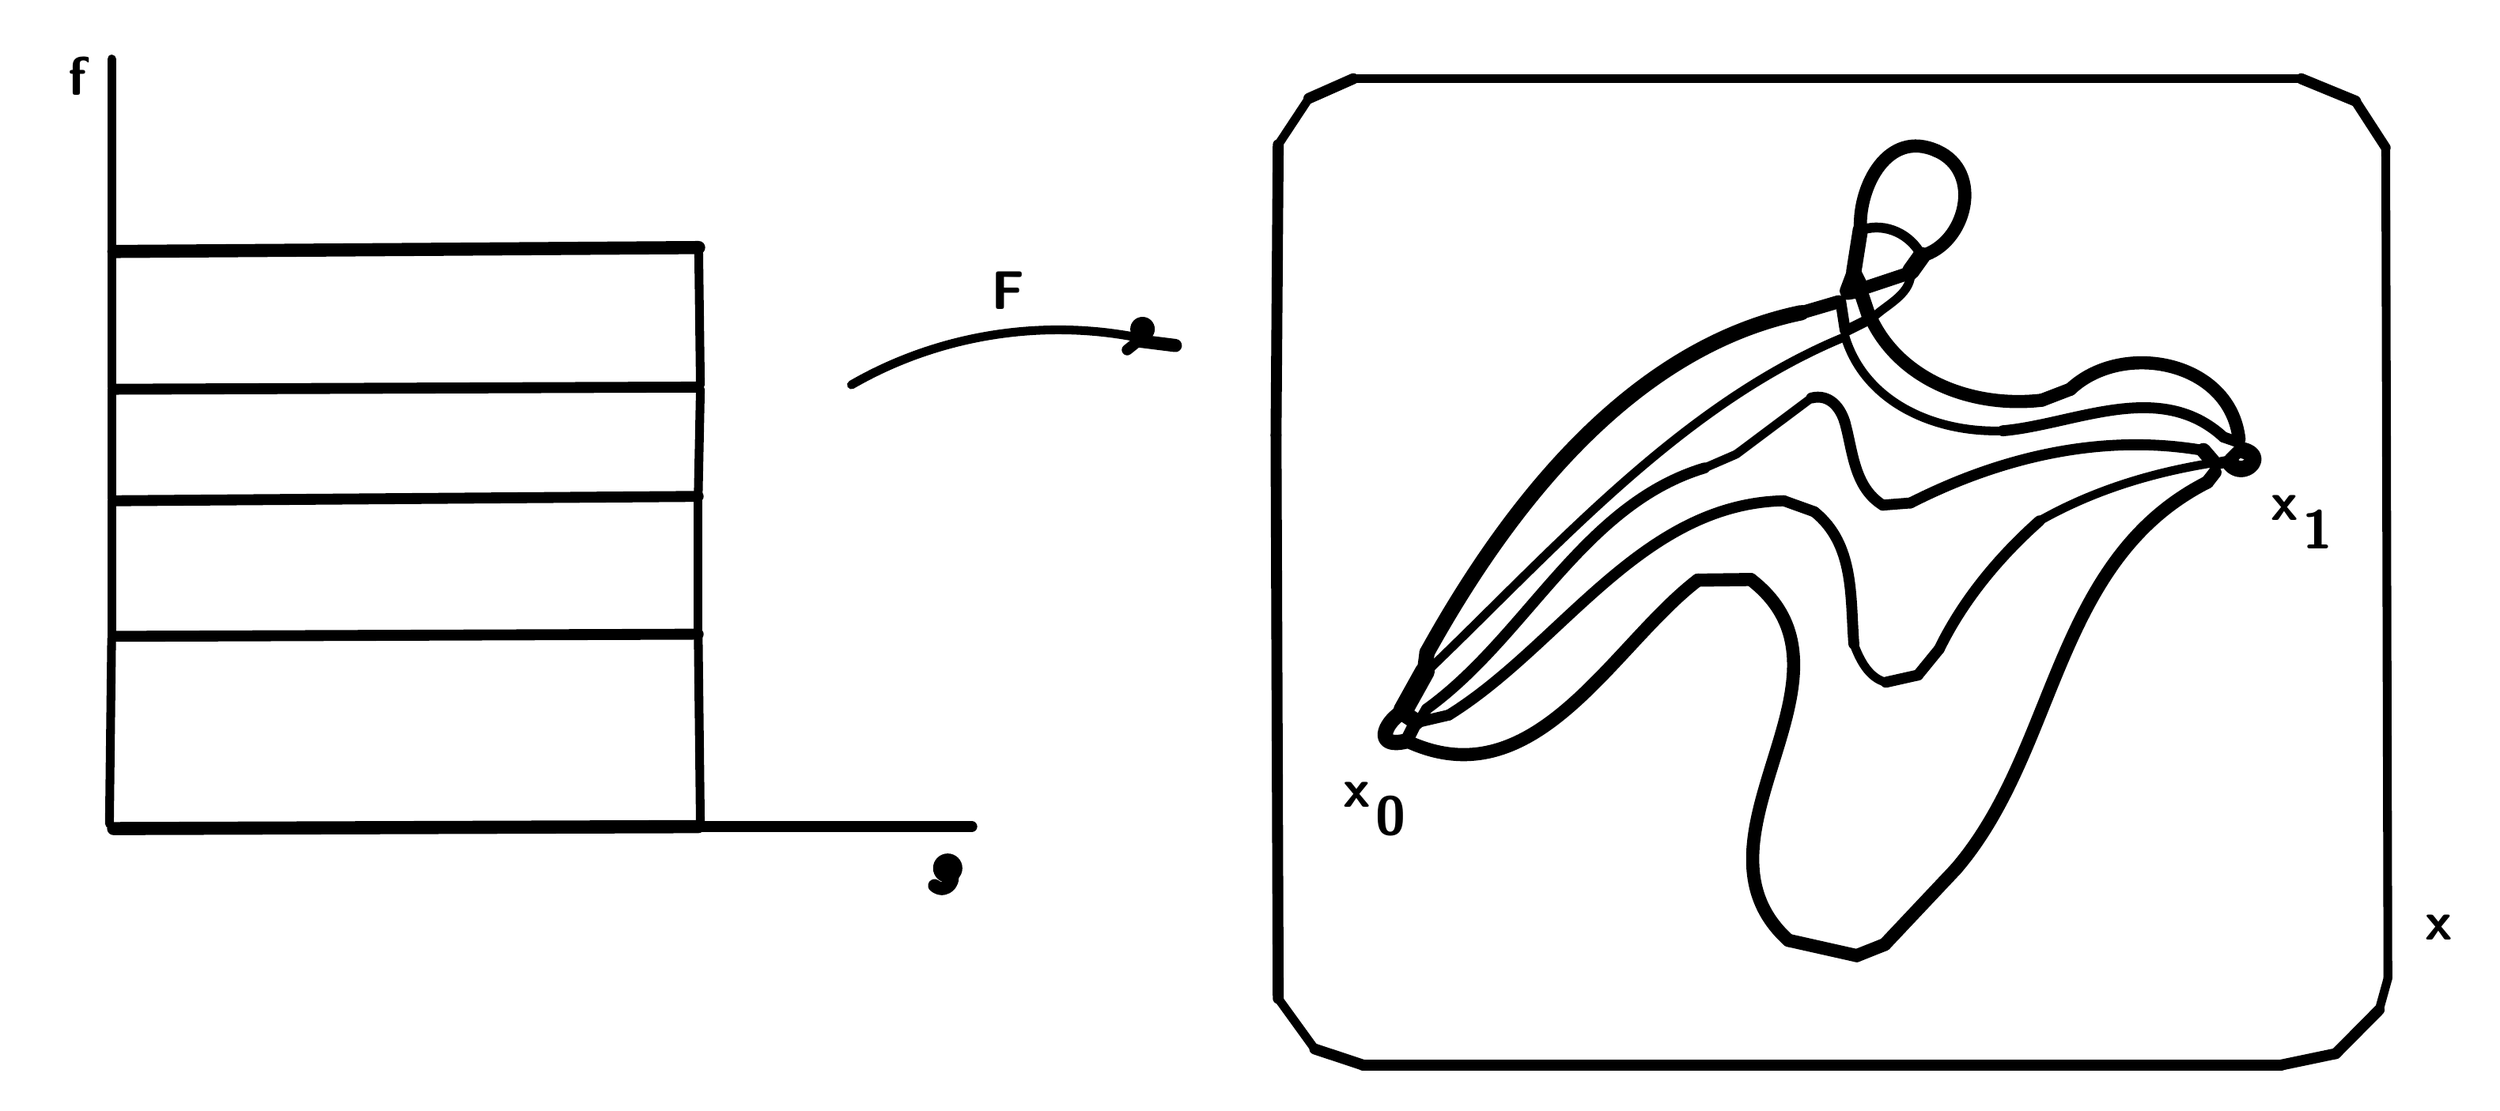
\begin{tikzpicture}[x=1pt, y=-1pt, line width=8.0pt, line cap=round, line join=round]

  %% ════ 填充区（prims2 的 fills）════

  %% ════ 直线段（prims2 的 strokes）════
  \draw[line width=8.0pt] (863.0,114.0) -- (868.0,107.0);
  \draw[line width=6.0pt] (862.0,115.0) -- (841.0,122.0);
  \draw[line width=7.0pt] (641.0,296.0) -- (642.0,288.4);
  \draw[line width=6.0pt] (813.0,133.0) -- (830.0,128.0);
  \draw[line width=6.0pt] (309.0,368.0) -- (41.9,368.9);
  \draw[line width=2.9pt] (41.9,368.9) -- (40.0,366.7);
  \draw[line width=4.0pt] (40.0,366.7) -- (41.0,282.0);
  \draw[line width=4.0pt] (310.0,367.0) -- (309.0,280.0);
  \draw[line width=5.0pt] (833.0,141.0) -- (831.0,128.0);
  \draw[line width=4.0pt] (41.0,281.0) -- (41.0,219.0);
  \draw[line width=6.0pt] (527.0,148.0) -- (511.0,146.0);
  \draw[line width=6.5pt] (844.0,135.0) -- (840.0,123.0);
  \draw[line width=3.4pt] (1014.0,195.0) -- (1013.0,192.0);
  \draw[line width=5.7pt] (1013.0,196.0) -- (1009.0,200.0);
  \draw[line width=9.0pt] (631.0,315.0) -- (641.0,297.0);
  \draw[line width=4.0pt] (41.0,104.0) -- (41.0,17.0);
  \draw[line width=5.3pt] (1003.0,202.0) -- (1008.0,201.0);
  \draw[line width=7.0pt] (840.0,95.0) -- (837.0,114.0);
  \draw[line width=5.0pt] (1005.9,189.9) -- (1012.0,192.0);
  \draw[line width=6.0pt] (42.0,105.0) -- (309.2,103.2);
  \draw[line width=4.0pt] (309.2,103.2) -- (310.0,166.0);
  \draw[line width=5.0pt] (639.0,319.0) -- (641.8,314.2);
  \draw[line width=4.0pt] (768.8,204.0) -- (783.3,197.7);
  \draw[line width=4.0pt] (783.3,197.7) -- (817.6,172.0);
  \draw[line width=5.0pt] (850.2,221.0) -- (862.9,220.0);
  \draw[line width=6.8pt] (996.7,196.0) -- (1001.0,201.0);
  \draw[line width=6.3pt] (840.0,123.0) -- (834.0,124.0);
  \draw[line width=5.0pt] (836.0,115.0) -- (833.0,123.0);
  \draw[line width=6.0pt] (1002.0,206.0) -- (998.5,210.5);
  \draw[line width=6.0pt] (883.6,387.4) -- (851.1,421.9);
  \draw[line width=6.0pt] (851.1,421.9) -- (838.3,427.0);
  \draw[line width=6.0pt] (838.3,427.0) -- (807.1,420.0);
  \draw[line width=6.0pt] (789.9,255.0) -- (765.7,255.3);
  \draw[line width=4.0pt] (310.0,168.0) -- (309.0,217.0);
  \draw[line width=6.0pt] (922.9,173.0) -- (935.9,168.0);
  \draw[line width=6.0pt] (633.0,328.0) -- (637.0,320.0);
  \draw[line width=4.0pt] (41.0,218.0) -- (41.0,168.0);
  \draw[line width=5.0pt] (834.0,141.0) -- (844.0,136.0);
  \draw[line width=7.5pt] (631.0,316.0) -- (637.0,320.0);
  \draw[line width=5.0pt] (42.0,281.0) -- (309.0,280.0);
  \draw[line width=5.0pt] (510.0,146.0) -- (505.0,150.0);
  \draw[line width=5.0pt] (434.0,368.0) -- (310.0,368.0);
  \draw[line width=5.0pt] (42.0,219.0) -- (309.0,217.0);
  \draw[line width=7.1pt] (840.0,121.0) -- (837.0,115.0);
  \draw[line width=5.0pt] (309.0,167.0) -- (42.0,168.0);
  \draw[line width=4.0pt] (41.0,106.0) -- (41.0,167.0);
  \draw[line width=4.0pt] (309.0,280.0) -- (309.0,217.0);
  \draw[line width=5.0pt] (876.0,286.8) -- (866.3,298.7);
  \draw[line width=5.0pt] (866.3,298.7) -- (851.6,302.0);
  \draw[line width=5.0pt] (818.9,224.0) -- (805.0,219.0);
  \draw[line width=5.0pt] (651.9,317.0) -- (639.0,320.0);
  \draw[line width=5.0pt] (573.0,189.0) -- (574.0,56.2);
  \draw[line width=4.0pt] (574.0,56.2) -- (588.0,35.0);
  \draw[line width=5.0pt] (588.0,35.0) -- (608.3,26.0);
  \draw[line width=4.0pt] (608.3,26.0) -- (1041.4,26.0);
  \draw[line width=5.0pt] (1041.4,26.0) -- (1066.2,36.2);
  \draw[line width=4.5pt] (1066.2,36.2) -- (1080.0,57.5);
  \draw[line width=4.0pt] (1080.0,57.5) -- (1081.0,437.4);
  \draw[line width=4.0pt] (1081.0,437.4) -- (1077.0,451.8);
  \draw[line width=5.0pt] (1077.0,451.8) -- (1057.2,471.8);
  \draw[line width=5.0pt] (1057.2,471.8) -- (1032.3,477.0);
  \draw[line width=5.0pt] (1032.3,477.0) -- (612.7,477.0);
  \draw[line width=5.0pt] (612.7,477.0) -- (590.7,469.7);
  \draw[line width=4.0pt] (590.7,469.7) -- (574.0,446.6);
  \draw[line width=5.0pt] (574.0,446.6) -- (573.0,189.0);

  %% ════ 曲线（prims2 的 curves —— 三段式，坐标同为 (y,x)）════
  \draw[line width=4.0pt] (863.0,116.0) .. controls (862.1,125.0) and (851.9,129.4) .. (846.0,135.0);
  \draw[line width=6.0pt] (423.0,387.0) .. controls (428.4,391.3) and (422.6,399.6) .. (417.0,395.0);
  \draw[line width=7.0pt] (642.0,288.4) .. controls (678.9,221.8) and (734.8,149.1) .. (813.0,133.0);
  \draw[line width=4.0pt] (642.0,297.0) .. controls (700.6,240.8) and (758.3,174.6) .. (833.0,144.0);
  \draw[line width=7.0pt] (630.0,316.0) .. controls (622.3,321.1) and (618.1,332.1) .. (632.0,329.0);
  \draw[line width=7.5pt] (1015.0,196.0) .. controls (1025.6,198.7) and (1014.9,209.2) .. (1009.0,202.0);
  \draw[line width=4.0pt] (833.0,144.0) .. controls (842.4,174.7) and (875.0,188.1) .. (905.0,187.0);
  \draw[line width=5.0pt] (905.0,187.0) .. controls (938.0,184.1) and (976.8,163.1) .. (1005.9,189.9);
  \draw[line width=5.0pt] (641.8,314.2) .. controls (687.7,281.0) and (713.2,220.7) .. (768.8,204.0);
  \draw[line width=5.0pt] (817.6,172.0) .. controls (825.8,170.0) and (830.7,176.2) .. (832.8,182.8);
  \draw[line width=5.0pt] (832.8,182.8) .. controls (836.6,196.1) and (836.9,212.7) .. (850.2,221.0);
  \draw[line width=5.0pt] (862.9,220.0) .. controls (903.5,199.3) and (950.0,187.9) .. (996.7,196.0);
  \draw[line width=6.0pt] (998.5,210.5) .. controls (927.8,246.4) and (930.5,332.7) .. (883.6,387.4);
  \draw[line width=6.0pt] (807.1,420.0) .. controls (755.8,373.4) and (847.0,299.0) .. (789.9,255.0);
  \draw[line width=6.0pt] (765.7,255.3) .. controls (726.6,285.2) and (691.5,356.2) .. (633.0,329.0);
  \draw[line width=4.0pt] (508.0,144.0) .. controls (463.3,135.7) and (417.0,144.0) .. (379.0,166.0);
  \draw[line width=6.0pt] (845.0,136.0) .. controls (858.9,164.9) and (892.6,176.6) .. (922.9,173.0);
  \draw[line width=6.0pt] (935.9,168.0) .. controls (959.8,145.5) and (1009.2,155.1) .. (1013.0,191.0);
  \draw[line width=4.5pt] (868.0,107.0) .. controls (863.0,97.1) and (851.6,91.7) .. (841.0,95.0);
  \draw[line width=6.0pt] (868.0,107.0) .. controls (888.3,101.4) and (896.6,68.5) .. (874.9,59.0);
  \draw[line width=6.0pt] (874.9,59.0) .. controls (852.5,48.9) and (839.3,75.2) .. (840.0,94.0);
  \draw[line width=4.0pt] (999.0,202.0) .. controls (971.9,206.5) and (945.8,214.6) .. (921.8,228.2);
  \draw[line width=5.0pt] (921.8,228.2) .. controls (902.9,245.0) and (886.7,264.8) .. (876.0,286.8);
  \draw[line width=4.0pt] (851.6,302.0) .. controls (843.7,300.0) and (839.6,291.5) .. (837.0,284.5);
  \draw[line width=5.0pt] (837.0,284.5) .. controls (835.3,263.1) and (837.5,238.9) .. (818.9,224.0);
  \draw[line width=5.0pt] (805.0,219.0) .. controls (739.5,220.4) and (703.3,285.1) .. (651.9,317.0);

  %% ════ 实心点 ════
  \fill (512.0,140.5) circle (5.6);
  \fill (423.0,387.0) circle (6.7);

  %% ════ 标签（probe 直接给的 \node 行）════
  %% ⚠ 全部补了 fill=white：文字在最上层，否则与曲线交叉干扰
     \node[anchor=center,inner sep=0pt,fill=white,font=\fontsize{26.5}{33.1}\selectfont] at (26.4,24.9) {\textsf{\textbf{\textit{f}}}};   % box(21,14,10,21)
     \node[anchor=center,inner sep=0pt,fill=white,font=\fontsize{30.0}{37.4}\selectfont] at (450.5,123.0) {\textsf{\textbf{\textit{F}}}};   % box(441,111,19,22)
     \node[anchor=center,inner sep=0pt,fill=white,font=\fontsize{29.2}{36.5}\selectfont] at (1034.0,222.4) {\textsf{\textbf{\textit{x}}}};   % box(1025,212,16,17)
     \node[anchor=center,inner sep=0pt,fill=white,font=\fontsize{23.7}{29.7}\selectfont] at (1048.8,232.4) {\textsf{\textbf{1}}};   % box(1042,224,8,16)
     \node[anchor=center,inner sep=0pt,fill=white,font=\fontsize{29.2}{36.5}\selectfont] at (610.0,353.4) {\textsf{\textbf{\textit{x}}}};   % box(601,343,16,17)
     \node[anchor=center,inner sep=0pt,fill=white,font=\fontsize{23.1}{28.9}\selectfont] at (625.4,363.2) {\textsf{\textbf{0}}};   % box(618,355,11,16)
     \node[anchor=center,inner sep=0pt,fill=white,font=\fontsize{38.0}{47.5}\selectfont] at (1104.3,414.0) {\textsf{\textbf{\textit{x}}}};   % box(1093,400,20,23)

  % 钉死画布：否则超出的图元/控制点会把页面撑大，1:1 回比就失准
  \pgfresetboundingbox
  \path[use as bounding box] (0,0) rectangle (1122,488);
\end{tikzpicture}
\end{document}

% ⚠ 待核清单（probe 拿不准，人眼过一遍）：
%   · 未识别/跳过：⑤ 跳过/未识别的字形
